\documentclass{standalone}
\usepackage{tikz}

\usetikzlibrary{calc,math}


\begin{document}

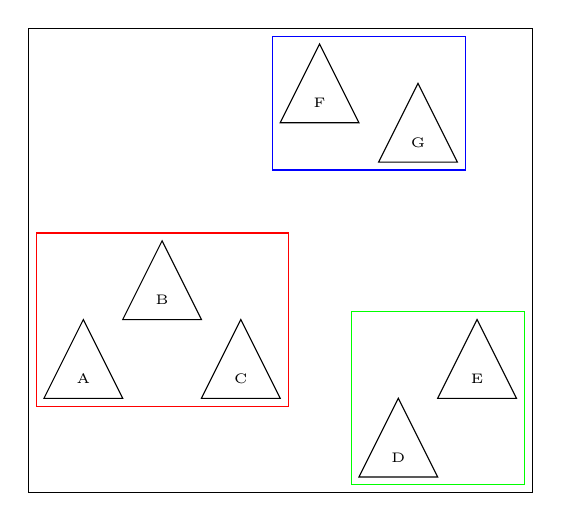
\begin{tikzpicture}
  \draw (0,0) -- (1,0) -- (0.5,1) -- cycle;
  \node[font=\tiny] at (0.5,0.25) { A };

  \begin{scope}[xshift=1cm,yshift=1cm]
    \draw (0,0) -- (1,0) -- (0.5,1) -- cycle;
    \node[font=\tiny] at (0.5,0.25) { B };
  \end{scope}

  \begin{scope}[xshift=2cm]
    \draw (0,0) -- (1,0) -- (0.5,1) -- cycle;
    \node[font=\tiny] at (0.5,0.25) { C };
  \end{scope}

  \begin{scope}[xshift=4cm,yshift=-1cm]
    \draw (0,0) -- (1,0) -- (0.5,1) -- cycle;
    \node[font=\tiny] at (0.5,0.25) { D };
  \end{scope}

  \begin{scope}[xshift=5cm]
    \draw (0,0) -- (1,0) -- (0.5,1) -- cycle;
    \node[font=\tiny] at (0.5,0.25) { E };
  \end{scope}

  \begin{scope}[xshift=3cm,yshift=3.5cm]
    \draw (0,0) -- (1,0) -- (0.5,1) -- cycle;
    \node[font=\tiny] at (0.5,0.25) { F };
  \end{scope}

  \begin{scope}[xshift=4.25cm,yshift=3cm]
    \draw (0,0) -- (1,0) -- (0.5,1) -- cycle;
    \node[font=\tiny] at (0.5,0.25) { G };
  \end{scope}

  \draw[red] (-0.1,-0.1) rectangle (3.1,2.1);
  \draw[green] (3.9,-1.1) rectangle (6.1,1.1);
  \draw[blue] (2.9,2.9) rectangle (5.35,4.6);
  \draw (-0.2,-1.2) rectangle (6.2,4.7);
\end{tikzpicture}

\end{document}
